\documentclass[12pt]{article}
\usepackage{amsfonts, amssymb, amsmath, amsthm, enumerate, multicol, xspace, array, multirow, graphicx, hyperref}
\begin{document}
\title{112 TP1 Design Proposal}
\author{Ethan Lu, AndrewID: ethanlu}
\maketitle
\section{Project Overview}

\subsection{Project Description}
    Overall, the goal of this project is to provide a useful and fluid framework for performing style transfer in real time through modification of game assets and textures. 
    Most notably, this project is designed to have novel applications for both game development and fan mods, which motivate much of the project's design. \\
    That's quite a wordy introduction though, so let's break down the various terms and components of the project:

    \subsubsection{Style Transfer:}
    A cool subset of Machine Learning/Deep Learning that seeks to quantify the ``style" or an image or painting, then apply it to other images. 
    For this project, I'm interested in realizing these algorithms in real time.\\
    Examples: \\
    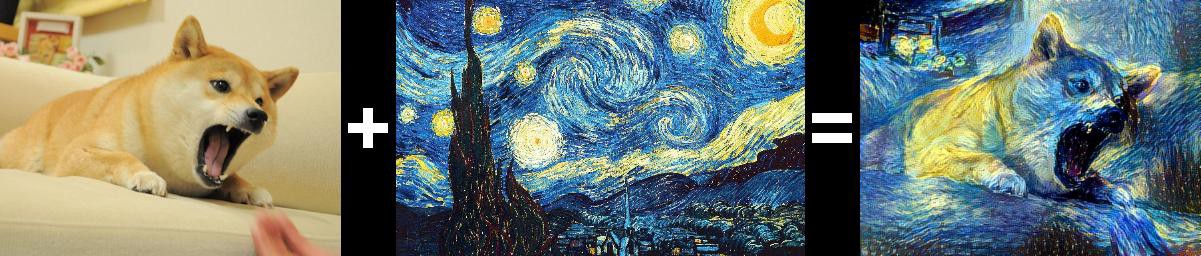
\includegraphics[width=\columnwidth]{ex1.jpg}\\
    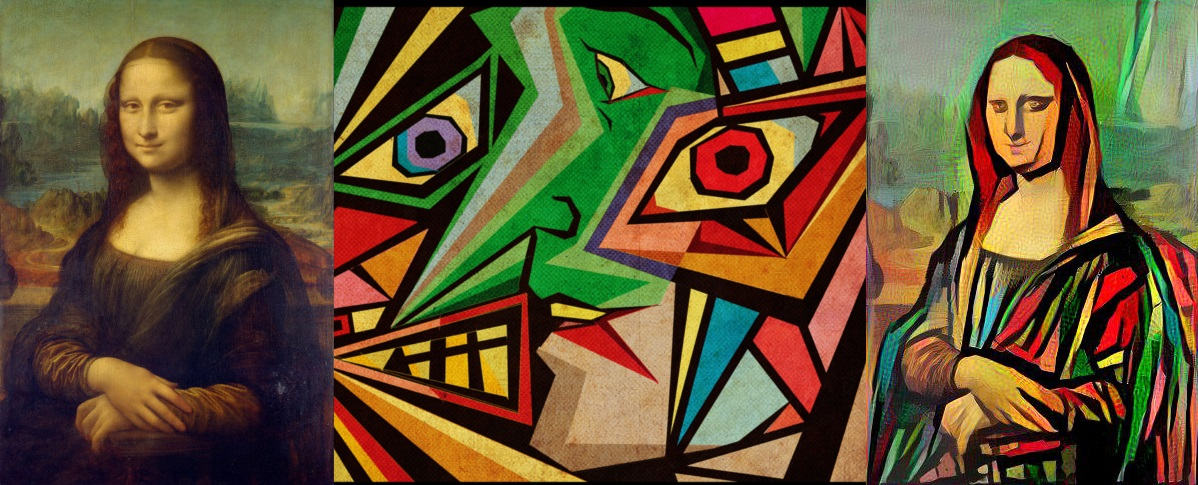
\includegraphics[width=\columnwidth]{ex2.jpg}

    \subsubsection{Issues with generalized style transfer algorithms for real time video}
    
    Very computationally expensive. For arbitrary video streams, based on the algorithm used, single frames can take anywhere from seconds to minutes to process, even on (very) good hardware.
    Also, these algorithms don't preserve temporal coherence, frequently resulting in flickering between frames. 

    My project aims to implement real-time style transfer on a very narrow subset of ``arbitrary video streams:" video games.

    Eseentially, I'm taking advantage of the fact that the output of video games is algorithmically generated, computationally using a combination of in-game models and textures to specify the content of each image.
    Thus, we can ``style transfer" onto the assets/textures used by the game, effectively getting similar results. 
    Analogy: doing style transfer at ``compile-time" instead of ``run-time."

\subsection{Competitive Analysis}
    As mentioned above, most of the existing solutions out there are extremely computationally demanding.
    The only working demo that does style transfer in remotely real time is \href{https://www.youtube.com/watch?v=vAelubuwquE}{NVIDIA's demo}, which requires 4x Titan Vs, something far beyond a typical workstation.
    
    Furthermore, it doesn't seem like anyone has attempted to apply style transfer to video games at all, which means this project represents something entirely new.
\subsection{Structural Plan}
    In terms of code, my source files will be divided into three primary files:
    \begin{enumerate}
        \item application.py: Implements the main user interface in QT. Handles function calls and other changes as necessary.
        \item alg.py: The actual implementations of the two algorithms described above.
        \item fileManager.py: Various utility functions that are used throughout the previous two files, with a particular emphasis on file system management.
    \end{enumerate}
\subsection{Algorithmic Plan}

    \subsubsection{Terms:}
    Style Image: the image from which the ``Style" of the desired output image is extracted\\
    Input/Content Image: the image that dictates the ``content" and overall geometry of the desired output image\\

    \subsubsection{Convolutional Neural Network + Gradient Descent:}
    Using a pretrained neural network (traditionally, vgg16/vgg19), we can quantify ``style" and ``content" differences between two image by looking at various layers of the convolution. To do this, we simply run each image through the neural network, examine the desired layer, and take the RMS difference between each component in the tensor. 
    This gives us two different notions of ``distance": style distance and content distance. Our goal is to minimize these. 

    To do this, we simply compute the gradients of each entry of the ``image tensor," and perform gradient descent on the entire tensor. 

    After the desired number of iterations, we return the output image and save it to a file.

    \subsubsection{Cycle GANs:}
    Two primary components:
    Generator 
    Discriminator
    First, we write a generator that naively does some basic operations on the input/style images. Most importantly, this generator is very fast, and can produce multiple images from a given pair of inputs very quickly. 

    Then, we write a discriminator that can pick the ``best" image out a set of candidate images, and run the generator again on this ``best" image. As part of the ``cycle" aspect, we also frequently regularize the outputs of this as to not get stuck in local maxima. 
    \subsubsection{Complete toolchain:}
    Main technologies: Pytorch, QT, Dolphin Emulator (for actually running the games). \\
    Workflow: \\
    (Optional/computationally demanding) Extract textures from the game using Dolphin Emulator, facilitated by a QT GUI. \\
    Parse the extracted textures from dolphin with Python builtin file operations \\
    Run the style transfer algorithms on above images with custom implementations in Pytorch \\
    Replace the original textures in dolphin \\
    Play the game again, using a button somewhere in the GUI. \\

\subsection{Timeline Plan}
    \textbf{TP1:} Have user interface/GUI designed and implemented. Seperately, have a working version of the convolutional NN algorithm.\\
    \textbf{TP2:} Bind the two together, add necessary filesystem manipulations to the GUI. Implement the cycle GAN algorithm.\\
    \textbf{TP3:} Add synthetic benchmarking and related graph/statistic visualization.\\
\subsection{Version Control Plan}
    I'll be using GitHub to backup/version control my code. 
    The repo I'll be using can be found at \href{https://github.com/elu00/112TP}{https://github.com/elu00/112TP}. \\
    
\includegraphics[scale=0.8]{screenshot.png}
\subsection{Module list}
\begin{enumerate}
	\item Pytorch/torchvision + PIL.
	\item PyQT for QT bindings/User Interface.
	\item Built-in Python packages (os, subprocess) for file manipulations.
\end{enumerate}
\subsection{TP2 Update}
	So far, I haven't needed to make any significant changes to my design plans.
\section{Storyboard}
See storyboard.png
\begin{enumerate}[(1)]
    \item The default user interface
    \item Styles can be dynamically changed using the dropdown menu
    \item After clicking "play game" ....
    \item Dolphin will launch with the modified textures
    \item If no preview image is available, fallback to the style image.
    \item New styles can also be added with an input image.
\end{enumerate}
\end{document}
